\documentclass[dissertation.tex]{subfiles}

\begin{document}

The compiler is comprised of a number of stages and substages, as shown in Figure \ref{fig:compiler-layout}:

\begin{figure}[h]
    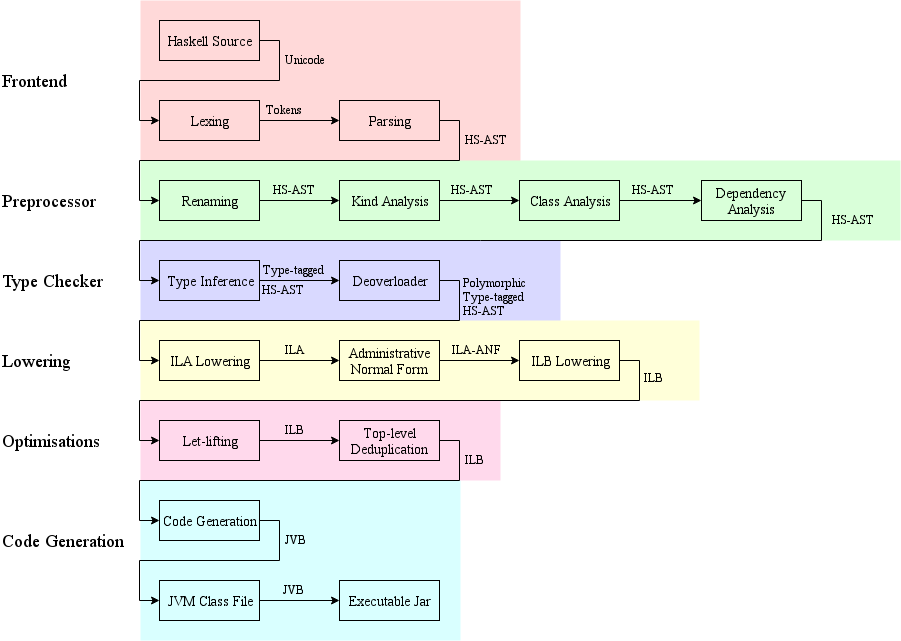
\includegraphics[width=\textwidth]{figures/compiler_layout.png}
    \caption{}
    \label{fig:compiler-layout}
\end{figure}

A brief overview of each stage is given here for a `big picture' view of the compiler, followed by more detailed
descriptions below.

\begin{description}
\item[Frontend]
{
    \hfill

    The frontend consists of standard lexing and parsing from Haskell source code into an Abstract Syntax Tree
    (AST). A modified version of an existing library (haskell-src\footnote{https://github.com/hnefatl/haskell-src})
    is used.

}
\item[Preprocessing]
{
    \hfill
    \begin{itemize}
    \item
    {

        The renamer renames each variable so that later stages can assume each variable name is unique:
        this reduces complexity by removing the possibility of variable shadowing (eg.\ \haskell{let x = 1 in let x = 2 in x}).

    }
    \item
    {

        Kind and Class analysis both simply extract useful information about the declarations in the source so that
        stages of the type checker are simpler.

    }
    \item
    {

        Dependency analysis computes a partial order on the source declarations so that the typechecker can process
        them in a valid order.

    }
    \end{itemize}
}
\item[Type Checker]
{
    \hfill
    \begin{itemize}
    \item
    {

        The type inference stage infers polymorphic overloaded types for each symbol, checks them against any
        user-provided type signatures, and alters the AST so that each expression is tagged with its type.

    }
    \item
    {

        Deoverloading converts polymorphic overloaded types to polymorphic types similar to those of System F, and
        alters the AST to implement typeclasses using dictionary-passing.

    }
    \end{itemize}
}
\item[Lowering]
{
    \hfill

    The lowering stage transforms the Haskell source AST into Intermediate Language A (ILA), then rearranges that
    tree into Administrative Normal Form (ILA-ANF), before finally transforming it into Intermediate Language B
    (ILB).

}
\item[Optimisations]
{
    \hfill

    Optimisations transform the intermediate languages into more efficient forms while preserving their semantics.

    \todo[inline]{At time of writing these are done on ILB, might change to ILAANF so should update this accordingly.}
    \todo[inline]{If any more optimisations are implemented, update the diagram and here.}

}
\item[Code Generation]
{
    \hfill

    ILB is transformed into Java Bytecode (JVB), and a modified version of an existing library
    (hs-java\footnote{https://github.com/hnefatl/hs-java}) is used to convert a logical representation of the
    bytecode into a set of class files, which are then packaged into an executable Jar file.

}
\end{description}


\section{Implementation Details}
{
    \subsection{Frontend}
    {

        Lexing and parsing of Haskell source is performed using the
        \monospace{haskell-src}\footnote{https://hackage.haskell.org/package/haskell-src} library, which I have modified
        to provide some additional desirable features:

        \begin{itemize}
        \item
        {
            Lexing and parsing declarations for built-in constructors like list and tuple definitions (eg.\
            \haskell{data [] a = [] | a:[a]}).
        }
        \item
        {
            Parsing data declarations without any constructors (eg.\ \haskell{data Int})\footnote{Declarations of this
            form are invalid in the original Haskell 1998 syntax, but valid in Haskell 2010: see
            https://wiki.haskell.org/Empty\_type}. This is a valuable way of introducing built-in types.
        }
        \item
        {
            Adding \haskell{Hashable} and \haskell{Ord} typeclass instances to the syntax AST, so that syntax trees can
            be stored in associative containers.
        }
        \end{itemize}

        The syntax supported is a strict superset of Haskell 1998 and a strict subset of Haskell 2010, but my compiler
        does not have support for all of the features implied by the scope of the syntax. For example, multi-parameter
        typeclasses are parsed correctly as a feature of Haskell 2010 but get rejected by the deoverloading stage.

        \begin{figure}[h]
            \begin{haskellfigure}
            class Convertable a b where
                convert :: a -> b
            instance Convertable Bool Int where
                convert True = 1
                convert False = 0
            \end{haskellfigure}
            \caption{An example of a multi-parameter typeclass}
        \end{figure}

    }
    \subsection{Preprocessor}
    {

        The preprocessing passes either make the Haskell source easier to deal with by later passes, or extract useful
        information to prevent subsequent passes from needing to extract information while applying transformations.

        \subsubsection{Renaming}
        {

            Haskell allows for multiple variables to share the same name within different scopes, which can increase the
            complexity of later stages in the pipeline. For example, when typechecking the following code we might
            conflate the two uses of \haskell{x}, and erroneously infer that they have the same type. A similar problem
            arises with variable shadowing, when the scopes overlap. The problem also applies to any type variables
            present in the source -- the type variable \haskell{a} is distinct between the two type signatures:

            \begin{haskellfigure}
            id :: a -> a
            id x = x

            const :: a -> b -> a
            const x _ = x
            \end{haskellfigure}

            Additionally, variables and type variables are in different namespaces: the same token can refer to a
            variable and a type variable, even within the same scope. The following code is perfectly valid (but loops
            forever), despite the same name being used for a type variable and a variable:

            \begin{haskellfigure}
            x :: x
            x = x
            \end{haskellfigure}

            To eliminate the potential for subtle bugs stemming from this feature, the renamer pass gives each distinct
            variable/type variable in the source a unique name (in the above example, the variable \haskell{x} might be
            renamed to \haskell{v0} and the type variable renamed to \haskell{tv0}, provided those names haven't been
            already used).
            
            Unique variable/type variable names are generated by prefixing the current value of an incrementing counter
            with either \haskell{v} for variable names or \haskell{tv} for type variable names. The renamer traverses
            the syntax tree maintaining a mapping from a syntactic variable/type variable name to an associated stack of
            unique semantic variable names (in Haskell, a \haskell{Map VariableName [UniqueVariableName]}):

            \begin{itemize}
            \item When processing the binding site of a new syntactic variable (eg.\ a let binding, a lambda argument, a
            pattern match...), a fresh semantic name is generated and pushed onto the stack associated with the
            syntactic variable.
            \item Whenever we leave the scope of a syntactic variable, we pop the top semantic name from the associated
            stack.
            \item When processing a use site of a syntactic variable, we replace it with the current top of the
            associated stack.
            \end{itemize}

            An analogously constructed mapping is maintained for type variables, but is kept separate from the variable
            mapping: otherwise the keys can conflict in code such as \haskell{x :: x}.

            Type constants, such as \haskell{Bool} from \haskell{data Bool = False | True} and typeclass names like
            \haskell{Num} from \haskell{class Num a where ...}, are not renamed: these names are already guaranteed to
            be unique by the syntax of Haskell, and renaming them means we need to maintain more mappings and carry more
            state through the compiler as to what they've been renamed to.

        }
        \subsection{Kind/Class Analysis}
        {

            The typechecker and deoverloader require information about the kinds of any type constructors (the `type of
            the type', eg.\ \haskell{Int :: *} and \haskell{Maybe :: * -> *}), and the methods provided by different
            classes. This is tricky to compute during typechecking as those passes traverse the AST in dependency order.
            Instead, we just perform a traversal of the AST early in the pipeline to aggregate the required information.

        }
        \subsection{Dependency Analysis}\label{sec:dependency-analysis}
        {

            When typechecking, the order of processing declarations matters: we can't infer the type of \haskell{foo =
            bar baz} until we've inferred the types of \haskell{bar} and \haskell{baz}. The dependency analysis stage
            determines the order in which the typechecker should process declarations.

            We compute the sets of free/bound variables/type variables/type constants for each declaration, then
            construct a dependency graph -- each node is a declaration, and there's an edge from \(A\) to \(B\) if any
            of the bound variables/type variables/type constants at \(A\) are free in \(B\). It is important to
            distinguish between variables/type variables and type constants, as otherwise name conflicts could occur (as
            we don't rename type constants). This separation is upheld in the compiler by using different types for
            each, and is represented in the dependency graph below by colouring variables red and constants blue.

            The strongly connected components of the dependency graph correspond to sets of mutually recursive
            declarations, and the partial order between components gives us the order to typecheck each set. For
            example, from the dependency graph in Figure \ref{fig:dependency-graph} we know that: we need to typecheck
            \(d_3\), \(d_4\), and \(d_5\) together as they're contained within the same strongly-connected component so
            are mutually recursive; we have to typecheck \(d_2\) last, after both other components.

            \begin{figure}[h]
            \centering
            \begin{subfigure}[b]{0.45\textwidth}
                \begin{haskellfigure*}{linenos=false}
                data Bool = False | True      #\(d_1\)#
                x = f True                    #\(d_2\)#
                f y = g y                     #\(d_3\)#
                g y = h y                     #\(d_4\)#
                h y = f y                     #\(d_5\)#
                \end{haskellfigure*}
            \end{subfigure}
            \begin{subfigure}[b]{0.5\textwidth}
                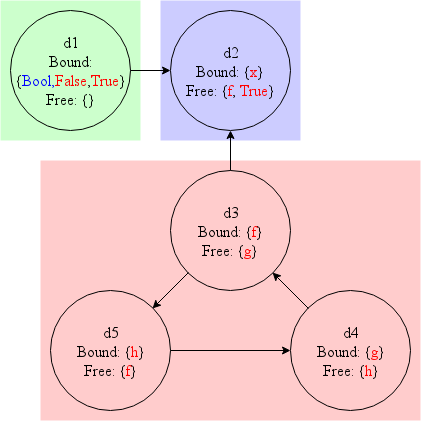
\includegraphics[width=\textwidth]{figures/dependency_graph.png}
            \end{subfigure}
            \caption
            {
                Code labelled with declaration numbers, and the corresponding dependency graph. Variables are
                in red text, type constants in blue. Strongly connected components are highlighted.
            }
            \label{fig:dependency-graph}
            \todo[inline]{Prettier graph: better colours/some other grouping style, and use a more latex-y font.}
            \end{figure}

            Typechecking declarations within the same component can proceed in an arbitrary order, we just need to
            ensure that the all of the type variables for the names bound by the declarations are available while
            processing each individual declaration.

            This process works for languages without ad-hoc overloading, like SML. However, in Haskell there are some
            complications introduced by typeclasses:

            \begin{itemize}
            \item
            {
                Typeclass member variables can be declared multiple times within the same scope. For example:
                
                \begin{haskellfigure}
                class Num a where
                    (+) :: a -> a -> a
                instance Num Int where
                    x + y = ...
                instance Num Float where
                    x + y = ...
                \end{haskellfigure}

                Here the multiple declarations of \haskell{+} don't conflict: this is a valid program. However, the
                following program does have conflicting variables, as \haskell{x} is not a typeclass member and is not
                declared inside an \haskell{instance} declaration:

                \begin{haskellfigure}
                x = True
                x = False
                \end{haskellfigure}

                These declaration conflicts can be expressed as a binary symmetric predicate on declarations, as
                presented in Figure \ref{fig:conflict-grid}, where:

                \begin{itemize}
                \item
                {

                    \monospace{Sym #\(x\)#} and \monospace{Type #\(x\)#} represent top-level declaration and
                    type-signature declarations for a symbol \(x\), like \haskell{#\(x\)# = True} and \haskell{#\(x\)# :: Bool}.

                }
                \item
                {
                    
                    \monospace{ClassSym #\(x\)# #\(c\)#} and \monospace{ClassType #\(x\)# #\(c\)#} represent
                    \monospace{Sym #\(x\)#} and \monospace{Type #\(x\)#} inside the declaration for a class \(c\), like
                    \haskell{class #\(c\)# where { #\(x\)# = True ; #\(x\)# :: Bool }}.

                }
                \item
                {

                    \monospace{InstSym #\(x\)# #\(c\)# #\(t\)#} represents a \monospace{Sym #\(x\)#} inside the
                    declaration for a class instance \(c\;t\), like \haskell{instance #\(c\)# #\(t\)# where { #\(x\)# = True }}.

                }
                \end{itemize}

                \begin{figure}[h]
                \small
                \setlength{\tabcolsep}{2pt}
                \begin{tabular}{ l | c c c c c }
                & \texttt{Sym} \(x_1\) & \texttt{Type} \(x_1\) & \texttt{ClassSym} \(x_1\) \(c_1\) &
                \texttt{ClassType} \(x_1\) \(c_1\) & \texttt{InstSym} \(x_1\) \(c_1\) \(t_1\) \\
                \hline
                \texttt{Sym} \(x_2\) & \(x_1=x_2\) & \texttt{False} & \(x_1=x_2\) & \(x_1=x_2\) & \(x_1=x_2\) \\
                \texttt{Type} \(x_2\) & & \(x_1=x_2\) & \(x_1=x_2\) & \(x_1=x_2\) & \(x_1=x_2\) \\
                \texttt{ClassSym} \(x_2\) \(c_2\) & & & \(x_1=x_2\) & \(x_1=x_2 \wedge c_1 \neq c_2\) & \(x_1=x_2 \wedge c_1 \neq c_2\) \\
                \texttt{ClassType} \(x_2\) \(c_2\) & & & & \(x_1=x_2\) & \(x_1=x_2 \wedge c_1 \neq c_2\) \\
                \texttt{InstSym} \(x_2\) \(c_2\) \(t_2\) & & & & & \makecell{\(x_1=x_2 \wedge (c_1 \neq c_2 \vee t_1=t_2)\)}
                \\
                \end{tabular}
                \caption{The conflict relation: the bottom triangle is omitted as the predicate is symmetric}
                \label{fig:conflict-grid}
                \end{figure}

                Using this table we can see that the multiple declarations for \haskell{+} in the example above are
                \monospace{InstSym (+) Num Int} and \monospace{InstSym (+) Num Float} so do not conflict, while the
                declarations for \haskell{x} above are both \monospace{Sym x} so do conflict.

            }
            \item
            {

                Another complication introduced by typeclasses is that variable declarations such as \haskell{id = \\x
                -> x} are usually treated as being the unique binding definition of \haskell{id}, and any other uses
                within the same level of scope must be free rather than binding (otherwise we have conflicting
                definitions).
                
                However, we treat binding declarations inside \haskell{instance} declarations as actually being free
                uses rather than binding uses, so that the instance declaration forms a dependence on the class
                declaration where the variables are bound, ensuring it is typechecked first.

            }
            \item\label{sec:dependencies-syntactic-semantic}
            {

                The dependencies generated by this technique are \textit{syntactic}, not \textit{semantic}: this is a
                subtle but very important difference. The use of any ad-hoc overloaded variable generates dependencies
                on the class declaration that introduced the variable, but not the specific instance of the class that
                provides the definition of the variable used.

                \begin{haskellfigure}
                class Foo a where
                    foo :: a -> Bool
                instance Foo Bool where
                    foo x = x
                instance Foo [Bool] where
                    foo xs = all foo xs
                \end{haskellfigure}

                The declaration of \haskell{foo} in \haskell{instance Foo [Bool]} semantically depends on the specific
                overload of \haskell{foo} defined in \haskell{instance Foo Bool}, and yet no dependency will be
                generated between the two instances as neither declaration binds \haskell{foo} (\haskell{foo} is treated
                as being free within the declarations as described above): they will only generate dependencies to
                \haskell{class Foo a} (and to the declaration of \haskell{Bool} and \haskell{all}).

                Computing the semantic dependencies is too complicated to be done in this pass, so the problem is left
                and instead solved during the typechecking stage. A full explanation is given later, but the approach
                used is to defer typechecking instance declarations until a different declaration requires the
                information, and then attempt to typecheck the instance declaration then, in a Just-In-Time manner.

            }
            \end{itemize}
        }
    }
    \subsection{Type Checker}
    {

        Type inference and checking is the most complex part of the compiler pipeline. The type system implemented is
        approximately System \(\text{F}_\omega\) (the polymorphically typed lambda calculus with type constructors)
        along with algebraic data types, and type classes to provide ad-hoc overloading. The approximation is due to a
        number of alterations made by the Haskell Report to ensure that type inference is decidable.
        
        This is a subset of the type system used by GHC (System \(\text{F}_\text{C}\)), as that compiler provides
        extensions such as GADTs and type families requiring a more complex type system.

        \begin{haskellfigure}
        data TypeVariable = TypeVariable TypeVariableName Kind
        data TypeConstant = TypeConstant TypeVariableName Kind

        data Type = TypeVar TypeVariable
                  | TypeCon TypeConstant
                  | TypeApp Type Type Kind

        data Kind = KindStar
                  | KindFun Kind Kind
        \end{haskellfigure}

        A \haskell{Kind} is often described as the `type of a type': we say that \haskell{True :: Bool}, but looking to
        a type system `one level up' we can say \haskell{Bool :: #\(*\)#} where \(*\) is the type of a type constructor
        that takes no parameters. The type constructor \haskell{Maybe} has kind \(*\rightarrow*\), as it takes a single
        type parameter: applying it to a type of kind \(*\) yields a type of kind \(*\), such as
        \haskell{Maybe Int}. All Haskell values have a type with kind \(*\): there are no values for types of
        other kinds. Kinds are used in the type system to enforce type correctness (or perhaps kind correctness), such
        as rejecting \haskell{Bool Bool} as an invalid type application.

        Type variables have an associated kind to allow for type constraints such as \haskell{pure :: Functor #\(f\)# =>
        #\(\alpha\rightarrow f \alpha\)#}, which says that \haskell{pure} can take a value of any type and embed it into
        a functor parametrised by that type: \haskell{f} has kind \(*\rightarrow*\).

        A `simple type' is then represented as any tree of applications between type variables and type constants: these
        are types such as \haskell{Int -> Maybe Bool}. Haskell has more complex types, however: overloaded and
        polymorphic types.

        \begin{haskellfigure}
        data TypePredicate = IsInstance ClassName Type

        data Qualified a = Qualified (Set TypePredicate) a
        type QualifiedType = Qualified Type

        data Quantified a = Quantified (Set TypeVariable) a
        type QuantifiedType = Quantified QualifiedType
        type QuantifiedSimpleType = Quantified Type
        \end{haskellfigure}

        A qualified/overloaded type is a simple type with type constraints/predicates attached, such as \haskell{Eq
        #\(\alpha\)# => #\(\alpha\rightarrow\alpha\rightarrow\)# Bool} (the constraint here being just \haskell{Eq
        #\(\alpha\)#}). The constraints act as restrictions on the valid types that can fulfil the type variable, or
        equivalently predicates which must hold on the variables: the type signature is only valid for \(\alpha\) that
        are instance of the \haskell{Eq} typeclass.
        
        A quantified/polymorphic type is an overloaded type with a set of type variables that are universally quantified
        over the type, meaning they must later be instantiated to a specific type/type variable (universally quantified
        vaariables are `placeholder' variables). Haskell type signatures are implicitly quantified over all the
        contained type variables, but some extensions add explicit syntax: \haskell{id ::
        #\(\alpha\rightarrow\alpha\)#}, \haskell{id :: forall #\(\alpha\)#. #\(\alpha\rightarrow\alpha\)#}, and
        \haskell{id :: #\(\forall\alpha\)#. #\(\alpha\rightarrow\alpha\)#} all mean the same.

        During type inference, types are almost always polymorphic and often overloaded (\haskell{(==) :: forall
        #\(\alpha\)#. Eq #\(\alpha\)# => #\(\alpha\rightarrow\alpha\rightarrow\)# Bool}, \haskell{(+) :: forall
        #\(\alpha\)#. Num #\(\alpha\)# => #\(\alpha\rightarrow\alpha\rightarrow\alpha\)#}, \haskell{head ::
        [#\(\alpha\)#] -> #\(\alpha\)#}, ...). After deoverloading (section \ref{sec:deoverloading}), types are never
        overloaded. This difference is enforced by using \haskell{QuantifiedType} and \haskell{QuantifiedSimpleType}
        respectively.

        \todo[inline]{This is mentioned here as it's a good place to imply that things are really complicated and the following explanation makes simplifying assumptions, but it repeats stuff from the lexing+parsing section.}

        There are many types of `declaration' in the Haskell grammar: pattern bindings like \haskell{x = 1} and
        \haskell{(y, z@(Just w)) = (1, Just True)}, function definitions like \haskell{f x = x}, and even declarations
        which contain other declarations, such as class and instance declarations. In the following descriptions,
        `declaration' is assumed to refer to simple pattern binding declarations like \haskell{x = f y} unless otherwise
        mentioned: other declaration types are either easy to extend to, don't play much role in typechecking, or have
        complicated rules that \todo{that what?}

        \todo[inline]{Section giving overview of substitution and unification?}

        \subsubsection{Type Inference}
        {

            % Instance typing, with on-demand loading of instances. Refer back to renaming section
            % Mention Outside-In(X) as improvement

            The implementation is inspired by \cite{THIH} and uses similar rules as the Hindley-Milner (HM) type
            inference algorithm presented in \cite{HM-rules}. There are three passes over the source AST, each of which
            traverses the AST in dependency order as described in \ref{sec:dependency-analysis}.

            \begin{enumerate}
            \item
            {
                
                The first pass tags each subexpression with a type variable, then uses rules similar to the HM inference
                rules to infer the value of the type variable, usually using the type variables of subterms.
                
                Some expressions will generate constraints on type variables: using an overloaded function like
                \haskell{(+)} will first require instantiating the polymorphic type to an overloaded type
                (\(\forall\alpha.\;\text{Num}\alpha\Rightarrow\alpha\rightarrow\alpha\rightarrow\alpha\) to
                \(\text{Num}\beta\Rightarrow\beta\rightarrow\beta\rightarrow\beta\), where \(\beta\) is a fresh unique
                type variable), then moving the constraints from the type to the set of constraints built up while
                traversing this declaration to get just \(\beta\rightarrow\beta\rightarrow\beta\). This is the ground
                type that's unified with the type variable used to tag the use of \haskell{(+)}, and the constraint is
                stored for use after finishing traversing the declaration.

                After a pattern binding declaration has been fully traversed, types are generated for all the variable
                names bound by the patterns. This involves adding explicit quantifiers and constraints to the simple
                type inferred for the top-level expression on the right-hand-side of the binding. All free type
                variables in the simple type are added as universally quantified variables, and any constraints
                involving type variables that are free in the simple type are added as the qualifiers to the type.

                \todo[inline]{There should also be a check called the ambiguity check here, but I've not implemented it: it's a bit complicated and at the time I'd overshot my typechecking time budget by multiple weeks. Not having implemented it allows some invalid programs to get through the type system and crash at runtime :(. Not mentioning leaves an obvious gap for people who know this subject, should I say I've not implemented it?}

            }
            \item
            {

                The second pass simply traverses the AST again and updates the type variables used to tag each with the
                final expression type generated by the unification during the first pass.
                
                This can't be done efficiently during the first pass: consider the expression \haskell{((+)#\(^{t_1}\)#
                x#\(^{t_2}\)#)#\(^{t_3}\)#} where the \(t_i\) are type variables tagging the expressions. Assume we've
                inferred that \haskell{x :: #\(\alpha\)#} and \haskell{(+) ::
                #\(\beta\rightarrow\beta\rightarrow\beta\)#} as described above, and that we've unified \(t_1\) and
                \(t_2\) with these types respectively. Inferring the type of the overall expression would proceed by
                unifying the type of the first formal argument of the function (\(\beta\)) with the first actual
                argument (\(\alpha\)), and then using this substitution to type the return value of the function as
                \(\alpha\rightarrow\alpha\rightarrow\alpha\), which we can now unify with \(t_3\). Had we previously
                updated the subterm's tags to be their inferred concrete types we'd now have to update them again:
                \(\beta\) is no longer used as it's been unified with \(\alpha\), but our subterms may still contains
                uses of it.

            }
            \item
            {

                The third pass checks that any user-provided type signatures (such as the user explicitly annotating
                \haskell{5 :: Float}) are valid compared to what was actually inferred: if the user-provided tag is more
                general than the inferred tag, we reject the program.

                This could be done during the second pass, but was kept as a distinct pass for clarity in the code.

            }
            \end{enumerate}

            One departure from conventional polymorphic type systems is that Haskell's type system restricts
            polymorphism for some terms: let-bound variables are polymorphic over all their free type variables, while
            function parameters are never polymorphic. In practice, this means that in the code below, \haskell{f ::
            #\(\forall \alpha.\;\alpha \rightarrow a\)#} whereas \haskell{g :: #\(\alpha \rightarrow \alpha\)#}. The
            difference in semantics ensures that type inference remains decidable.
 
            \begin{haskellfigure}
            let f x = x in const (f True) (f 1) :: Bool -- This is fine
            (\\g -> const (g True) (g 1)) (\x -> x)     -- This fails to typecheck
            \end{haskellfigure}

            \todo[inline]{Originally I had a big worked example here, but after refactoring the above I don't know if it's needed: depends on whether reading the above makes sense or whether a continuous worked example would make it clearer.}

            A tricky part of the typechecking process is dealing with typeclasses, as dependency order isn't
            semantically accurate for typeclass instance declarations: the problem is detailed in
            \ref{sec:dependencies-syntactic-semantic}. To handle the potential issues, such declarations are processed
            in a lazy manner. If a declaration requires an instance of a typeclass in order to typecheck then that
            typeclass is typechecked immediately, and all remaining instance declarations are processed after
            non-instance declarations have been processed.

            An improvement to the current approach would be to implement the OutsideIn(X) framework given in
            \cite{OutsideIn}. This framework can work with Hindley-Milner type inference to handle more complex
            constraints than the current implementation, allowing support for GADTs and type families and handling type
            classes more flexibly than the current implementation.

        }
        \subsubsection{Deoverloader}\label{sec:deoverloading}
        {

            The deoverloading stage performs a translation which eliminates typeclasses, resulting in an AST tagged with
            types that no longer have type contexts. The implementation of typeclasses chosen was dictionary passing.

            To convert \haskell{add1 x = (+) x 1} with type \(\forall \alpha.\; \text{Num }\alpha \Rightarrow
            \alpha\rightarrow\alpha\) to a non-overloaded function, we can add an extra argument that carries the
            `implementation' of the \(\text{Num }\alpha\) constraint, which we then pass down to the \haskell{+}
            function: \haskell{add1' dNum x = (+) dNum x 1}.

            \todo[inline]{Alternative approaches than dictionary passing?}

            The approach used here is to perform a source-to-source transformation on the AST that replaces
            typeclass/instance declarations with datatype/value/function declarations.

            \begin{haskellfigure}
            class Eq a where
                (==), (/=) :: a -> a -> Bool
            instance Eq Bool where
                (==) = ...
                (/=) = ...
            \end{haskellfigure}

            Typeclasses are replaced by datatypes equivalent to tuples with an element for each function defined by the
            class, and instances are replaced by values of the respective class' datatype, filling in the elements using
            the implementation provided by the instance declaration. Extractor functions are added which pull specific
            elements out of the datatype to get at the actual implementation of the function.

            \begin{haskellfigure}
            -- Implementation of the typeclass
            data Eq a = Eq (a -> a -> Bool) (a -> a -> Bool)

            -- The functions defined by the typeclass extract the implementation functions
            (==), (/=) :: Eq a -> a -> a -> Bool
            (==) (Eq eq _) = eq
            (/=) (Eq _ neq) = neq

            -- The implementation of the typeclass instance
            dEqBool :: Eq Bool
            dEqBool = Eq dEqBoolEq dEqBoolNeq

            -- The function implementations defined in the instance
            dEqBoolEq, dEqBoolNeq :: Bool -> Bool -> Bool
            dEqBoolEq = ...
            dEqBoolNeq = ...
            \end{haskellfigure}


            To deoverload declarations using overloaded values, we essentially convert declarations of functions with
            types like \(\text{Num}\;\alpha\Rightarrow\alpha\rightarrow\alpha\) to
            \(\text{Num}\;\alpha\rightarrow\alpha\rightarrow\alpha\): we replace typeclass constraints with formal
            arguments to carry the implementation dictionaries. Similarly when using an expression of overloaded type,
            we add an actual argument to the call site for each typeclass constraint to account for the extra arguments
            we added to the definition.
            
            For example, \haskell{foo x = x == 1} deoverloads to \haskell{add1 dEqa x = (==) dEqa x 1}: we add an extra
            formal argument to the function declaration, and insert it in the call site to \haskell{+}.

            In order to know what variables to insert at call sites, the names of in-scope variables holding values of
            typeclass implementations are stored while traversing the AST. Initially the mapping contains the ground
            instances provided by top-level instance declarations (eg.\
            \(\{\text{Num\;Int}\mapsto\texttt{dNumInt},\;\text{Eq\;Int}\mapsto\texttt{dEqInt},\;...\}\)), and we update
            it to include any in-scope extra arguments we add to functions while deoverloading them. When we encounter
            an overloaded variable, we insert arguments for each type constraint by finding matching constraints within
            our mapping.

            One special case in the process is the handling of literals. Whilst arbitrary expressions with overloaded
            types always require a dictionary to be passed (consider that the innocent-looking \haskell{x} in
            \haskell{let x = 1 + 2 in x} involves an application of \haskell{+} which requires a dictionary to provide
            the implementation), literals do not require a dictionary as they can never perform any computation.

        }
    }
    \subsection{Lowering and Intermediate Languages}
    {

        There are two intermediate languages within the compiler, imaginatively named Intermediate Languages A and B
        (ILA and ILB respectively). There is also a minor language named ILA-Administrative Normal Form (ILA-ANF), which
        is simply a subset of ILA that helps restrict the terms to those in Administrative Normal Form (ANF).

        \todo[inline]{For each: why needed, BNF grammar, strengths. Probably don't go into details of translation?}

        \subsubsection{Intermediate Language A}
        {

            ILA is a subset of GHC's Core intermediate language, removing terms which are used for advanced language
            features like GADTs, as they are not supported by this compiler. Haskell 98 has hundreds of node types in
            its
            AST\footnote{\url{https://hackage.haskell.org/package/haskell-src/docs/Language-Haskell-Syntax.html}\todo[inline]{Find
            version-independent link}}, whereas ILA has far fewer: this makes it far easier to transform. Below is the
            full definition of ILA:

            \todo[inline]{Give BNF instead of Haskell ADTs?}
            \begin{haskellfigure}
            data Expr = Var VariableName Type
                      | Con VariableName Type
                      | Lit Literal Type
                      | App Expr Expr
                      | Lam VariableName Type Expr
                      | Let VariableName Type Expr Expr
                      | Case Expr [VariableName] [Alt Expr]
                      | Type Type

            data Literal = LiteralInt Integer
                         | LiteralChar Char

            data Alt a = Alt AltConstructor a

            data AltConstructor = DataCon VariableName [VariableName]
                                | Default

            data Binding a = NonRec VariableName a
                           | Rec (Map VariableName a)
            \end{haskellfigure}

            A Haskell program is lowered by this pass into a list of \haskell{Binding Expr}: a list of recursive or
            non-recursive bindings of expressions to variables.

            \todo[inline]{Use paragraph to split this into better titled chunks}

            One notable feature of ILA is that it carries type information: leaf nodes such as \monospace{Var} are
            tagged with a type. GHC's Core IL is fully explicitly typed under a variant of System F, which allows for
            `core linting' passes in-between transformations to ensure they maintain type-correctness. The type
            annotations on ILA are not sufficient for such complete typechecking, but do allow for some sanity checks
            and are necessary for lower stages of the compiler such as code generation. 

            ILA is still quite high-level, so many of the language constructs have similar semantics to their Haskell
            counterparts. The main benefit in this lowering pass is to collapse redundant Haskell syntax into a smaller
            grammar.

            Most of these constructors have obvious usages, but some are more subtle: \monospace{Con} represents a data
            constructor such as \haskell{True} or \haskell{Just}. \monospace{App} is application of expressions, which
            covers both function applications and data constructor applications (eg.\ \monospace{App (Var "f" (Bool
            #\(\rightarrow\)# Bool)) (Con "True" Bool)} and \monospace{App (Con "Just" (Int #\(\rightarrow\)# Maybe
            Int)) (Var "x" Int)}).
            \todo[inline]{Work out why spacing is weird here}

            \monospace{Lam #\(x\ t\ e\)#} represents a lambda term like \(\lambda x : t.\;e\), and \monospace{Let #\(x\
            t\ e_1\ e_2\)#} represents a term like \(\text{let } x:t = e_1 \text{ in } e_2\).

            \todo[inline]{Lam and Let are most easily explained as lambda terms, but App is most easily demonstrated with some code, and the switch between explanation styles is a bit jarring.}
            
            \monospace{Case #\(e\ vs\ as\)#} represents a multi-way switch on the value of an expression \(e\) (the
            `head' or `scrutinee'), matching against a number of possible matches (`alts') from the list \(as\), where
            the evaluated value of \(e\) is bound to each of the variables in \(vs\). The additional binding variables
            can be useful when the scrutinee expression is reused within some number of the alts.

            \todo[inline]{\monospace{Type} isn't really used afaik, it's a leftover from when I was trying to do System F style types. Should see if I can remove it.}
            
            The alts in a \monospace{Case} expression, of the form \monospace{Alt #\(c\ b\)#}, match the value of
            evaluating the scrutinee against the data constructor \(c\), then evaluates the \(b\) from whichever alt
            matched. \monospace{AltConstructor} represents the potential matches: either a data constructor with a
            number of variables to be bound, or a `match-anything' default value.


            Many syntax features in Haskell are just syntactic sugar, and are simple to desugar (list literals like
            \haskell{[1, 2]} are desugared to \haskell{1:2:[]}). Others are slightly more involved, such as converting
            \haskell{if x then y else z} expressions into \haskell{case x of { True -> y ; False -> z }}
            (\haskell{Bool}is just defined as an ADT in Haskell, there's no special language support for it).

            % Begin pattern matching spiel
            Other language features are non-trivial to lower, such as the rich syntax Haskell uses for pattern matching.
            An example pattern match could be \haskell{Just x@(y:z) = Just [1, 2]}, binding \haskell{x = [1, 2]},
            \haskell{y = 1}, and \haskell{z = [2]}. Multiple pattern matches can also be related, as in function
            definitions:

            \begin{haskellfigure}
            f (x, Just y) = x + y
            f (x, Nothing) = x
            \end{haskellfigure}

            Additionally, pattern matches can occur in a number of places: pattern-binding declarations such as
            \haskell{let (x, y) = z in ...}, functions definitions like the example above, lambda expressions, and
            \haskell{case} expressions (\haskell{case Just 1 of { Nothing -> ... ; Just x -> ... }}). The heterogeneity
            of use sites demands a flexible approach to translating pattern matches that can be reused for each
            instance.

            My initial implementation worked correctly for single-pattern uses, such as the \haskell{let} example above,
            but didn't support multiple parallel patterns as used in \haskell{case} expressions and function
            definitions. The current implementation is now based off the approach given in Chapter 5 of
            \cite{ImplFunLang}, which is a more general version of my initial algorithm.

            \todo[inline]{Feel like this needs a little bit more. Probably give a very brief overview, explain that everything's converted into case statements in the end, etc.}

            Finally, note that in Haskell a pattern will eventually match against a data constructor, a literal, or
            anything (with the wildcard pattern \haskell{_}). However, in the grammar for ILA's
            \haskell{AltConstructor}, there's no constructor corresponding to literals. This is due to \haskell{case}
            expressions generally only making sense for data constructors, where there are a finite number of
            constructors to check a value against for a given datatype. On the other hand, literals normally have a
            cumbersomely large (or infinite) number of `constructors' (one can imagine the \haskell{Int} type, which is
            bounded, as being defined as \haskell{data Int = ... | -1 | 0 | 1 | ... }, but \haskell{Integer} cannot be
            defined in this way as it is unbounded). As a result, literals are `pattern matched' by using equality
            checks from the \haskell{Eq} typeclass: the expression \haskell{case x of { 0 -> y ; 1 -> z ; _ -> w }} is
            essentially translated to \haskell{if x == 0 then y else if x == 1 then z else w}, which is then lowered
            into \haskell{case} expressions match on \haskell{True} and \haskell{False} as described above.
            % End pattern matching spiel

        }
        \subsubsection{Intermediate Language A - Administrative Normal Form}
        {

            Administrative Normal Form (ANF) is a style of writing programs in which all arguments to functions must be
            trivial (a variable, literal, or other irreducible `value' like a lambda expression). ANF is an alternative
            to Continuation Passing Style (CPS) as a style of intermediate language but can perform transformations in a
            single pass that would take multiple passes on a CPS program\cite{ANF}.

            This compiler uses ANF as it lends itself well to conceptualising lazy evaluation: as each complex
            expression is referred to through a variable, if the expression is evaluated by one computation then all
            other references to the variable transparently reference the resulting value, rather than a duplicate of the
            computation.

            ILA-ANF is a subset of ILA which uses a more restricted grammar to enforce more invariants on the language
            and guide the AST into ANF. The full definition of ILA-ANF is given below, and reuses the definitions of
            \haskell{Binding} and \haskell{Alt} from ILA.

            In the case of ILA-ANF, `trivial' terms are taken to be variables, data constructors, and literals. Note
            that this excludes lambda terms, which is somewhat unusual. Instead, lambda terms must immediately be bound
            to a variable: this restriction is enforced by the \haskell{AnfRhs} term in the grammar below.

            \todo[inline]{Why lambda terms not trivial? General design-decision explanation. Makes thunk model explicit + easier to generate code?}

            \begin{haskellfigure}
            data AnfTrivial = Var VariableName Type
                            | Con VariableName Type
                            | Lit Literal Type
                            | Type Type

            data AnfApplication = App AnfApplication AnfTrivial
                                | TrivApp AnfTrivial

            data AnfComplex = Let VariableName Type AnfRhs AnfComplex
                            | Case AnfComplex Type [VariableName] [Alt AnfComplex]
                            | CompApp AnfApplication
                            | Trivial AnfTrivial

            data AnfRhs = Lam VariableName Type AnfRhs
                        | Complex AnfComplex
            \end{haskellfigure}

            An ILA program is lowered from a list of \haskell{Binding Expr} to a list of \haskell{Binding AnfRhs} by
            this pass. The translation is quite simple compared to the other lowering passes -- most of the terms are
            similar to those in ILA (including carrying type information), with notable exceptions being the
            introduction of \haskell{AnfApplication}, which restricts application arguments to purely trivial terms, and
            \haskell{AnfRhs}, to enforce that lambda terms can only be bound to variables.

        }
        \subsubsection{Intermediate Language B}
        {

            ILB is the final intermediate language of this compiler and is inspired by GHC's STG (Spineless Tagless
            G-Machine) IL. ILB maintains the ANF style from ILA-ANF. It has a number of extremely useful features for
            code generation: the only term that performs any evaluation of an expression is the \haskell{ExpCase #\(e\
            t\ vs\ as\)#} term (which evaluates \(e\) then branches to one of the \(as\)), and the only term which
            performs any memory allocation is the \haskell{ExpLit #\(v\ r\ e\)#} term, which allocates memory on the
            heap to represent a datatype/literal/uneveluated expression then evaluates \(e\).

            Additionally, this language makes lazy evaluation `explicit', in the sense that expressions to be evaluated
            are always encapsulated within an \haskell{RhsClosure} (thanks to ANF style which names each subexpression)
            that can be implemented as a not-yet-evaluated thunk.

            \begin{haskellfigure}
            data Arg = ArgLit Literal
                     | ArgVar VariableName

            data Exp = ExpLit Literal
                     | ExpVar VariableName
                     | ExpApp VariableName [Arg]
                     | ExpConApp VariableName [Arg]
                     | ExpCase Exp Type [VariableName] [Alt Exp]
                     | ExpLet VariableName Rhs Exp

            data Rhs = RhsClosure [VariableName] Exp
            \end{haskellfigure}

            ILB is similar in grammar to ILA-ANF, and the translation pass is relatively simple. There are some key
            differences between the languages, that reflect the changes from a relatively high-level IL down to a
            lower-level one:

            \todo[inline]{Didn't use bullet points for the previous IL explanations: change them?}
            \begin{itemize}
            \item
            {

                There are now two terms for applications, one for functions (\haskell{ExpApp}) and one for data
                constructors (\haskell{ExpConApp}). The distinction is necessary for code generation, when a function
                application results in a jump to new executable code while a constructor application creates a new heap
                object.

                \haskell{ExpConApp} also requires all its arguments to be present: it cannot be a partial application.
                Haskell treats datatype constructors as functions, so the following is a valid program:

                \begin{haskellfigure}
                data Pair a b = Pair a b
                x = Pair 1
                y = x 2
                \end{haskellfigure}

                At the implementation level however, functions and data constructors are necessarily very different, so
                distinguishing them within this IL makes code generation easier.

                \todo[inline]{Include how they're distinguished? Or too much detail?}

            }
            \item
            {

                Right-hand-side terms in ILA (\haskell{AnfRhs}) were either lambda expressions or a let-binding/case
                expression/\dots -- in ILB, the only right-hand-side term is a \haskell{RhsClosure}. A closure with no
                arguments is essentially a thunk, a term that exists purely to delay computation of an expression, while
                a closure with arguments is the familiar lambda term.

                ILB's \haskell{RhsClosure} takes a list of arguments, whereas ILA-ANF's lambda terms only take a single
                argument (multiple-argument functions are just nested single-argument lambdas). This is another
                translation aimed at making code generation easier. Single-argument lambdas allow for simpler logic when
                handling partial application in higher-level languages, but is inefficient in implementation. ILB is the
                ideal IL to perform this switch from the high-level convenient-to-modify grammar to a lower-level
                efficient representation.

            }
            \item
            {

                ILB only allows variables in many of the places where ILA-ANF allowed variables, literals, or 0-arity
                data constructors (like \haskell{True}). This is another step towards making laziness explicit, by
                keeping expressions simple so that only one step of the evaluation needs to happen at a time.

            }
            \end{itemize}

        }
    }
    \subsection{Code Generation}
    {
        \todo[inline]{Left optimisations until after codegen: cover the main pipeline first then the optional stages later?}
        
        Code generation is, from the surface, quite a mechanically simple process. ILB is a small language, so there
        aren't many terms to lower into bytecode. Implementing the semantics of these terms in Java Bytecode is complex,
        however.

        The \monospace{hs-java} library was used to provide a Haskell representation of bytecode that could then be
        serialised to a Java \monospace{.class} file, but a number of modifications were made to the library by me to
        add support for Java 8 features required by the compiler, as well as a number of smaller improvements: the
        forked project can be found at \url{https://github.com/hnefatl/hs-java}.

        A number of Java classes have been written to provide the `primitives' used by generated bytecode: including the
        implementation of Haskell's primitive datatypes like \haskell{Int} and \haskell{Char}, as well as the base class
        for all ADTs definable within the language (\monospace{BoxedData}, described later). The compiler is aware of
        these `builtin' classes and uses a set of `hooks' when generating code to provide Java implementations of
        Haskell functions. This is covered in more detail later.

        % - Hooks: implementing a haskell value with java code.

        \subsubsection{Weak Head Normal Form}
        {

            A Haskell expression is in weak head normal form (WHNF) if it is either a partially applied function
            (including lambda terms), a fully/partially applied data constructor, or a literal. Any arguments need not
            have been evaluated.
            
            Evaluation of an expression up to WHNF corresponds to a form of non-strict evaluation: partial applications
            of functions or any data constructor applications don't force their arguments to be evaluated, but when a
            function is applied to all its arguments, it reduces to the body without necessarily having evaluated its
            arguments. In particular, the evaluation of a Haskell program is equivalent to evaluation to WHNF.

            The following Haskell expressions are either valid or invalid WHNF terms, as indicated:

            \begin{haskellfigure}
            1               -- In WHNF
            (+) 1           -- In WHNF
            1 + 2           -- Not in WHNF
            3               -- In WHNF
            Just            -- In WHNF
            Just True       -- In WHNF
            (\\x -> x) 1    -- Not in WHNF
            (+) (1 + 2)     -- In WHNF
            (1 + 2) + 3     -- Not in WHNF
            \end{haskellfigure}
        }
        \subsubsection{Heap Objects}
        {

            Literals, datatype values and closures are all represented at runtime by values on the heap, as they are all
            first-class values in Haskell, and will be referred to as `objects': this intentionally overloads the
            terminology used by Java for an instance of a class, as the two concepts are essentially interchangeable
            here as Java objects are heap-allocated.

            Thunks are represented simply as closures without arguments: all of the closure logic described below is the
            same between thunks and functions.

            All objects on the heap inherit from a common abstract base class, \java{HeapObject}:

            \begin{javafigure}
            public abstract class HeapObject implements Cloneable {
                public abstract HeapObject enter();

                @Override
                public Object clone() throws CloneNotSupportedException {
                    return super.clone();
                }
            }
            \end{javafigure}

            The abstract \java{enter} method evaluates the object to WHNF and returns a reference to the result, and the
            \java{clone} method simply returns a shallow copy of the object. This method is critically for implementing
            function applications, described later.

            \paragraph*{Literals}\label{sec:literals}
            {
                
                Literals are builtin types that can't be defined as an Haskell ADT, such as \haskell{Int}. Any such type
                is a subclass of the \java{Data} class, which is itself a subclass of the \java{HeapObject} class that a
                rather boring implementation of the abstract \java{enter} method. Any literal is already in WHNF, so
                evaluation to WHNF is trivial:

                \begin{javafigure}
                public abstract class Data extends HeapObject {
                    @Override
                    public HeapObject enter() {
                        return this;
                    }
                }
                \end{javafigure}

                Here is an example literal implementation for \haskell{Integer}, Haskell's arbitrary precision integral
                value type. It is implemented using Java's \java{BigInteger} class to perform all the computation. The
                copious uses of underscores is explained in the JVM Sanitisation section below.

                \begin{javafigure}
                import java.math.BigInteger;

                public class _Integer extends Data {
                    public BigInteger value;
                    public static _Integer _make_Integer(BigInteger x) {
                        _Integer i = new _Integer();
                        i.value = x;
                        return i;
                    }
                    public static _Integer _make_Integer(String x) {
                        return _make_Integer(new BigInteger(x));
                    }

                    public static _Integer add(_Integer x, _Integer y) {
                        return _make_Integer(x.value.add(y.value));
                    }
                    public static _Integer sub(_Integer x, _Integer y) { ... }
                    public static _Integer mult(_Integer x, _Integer y) { ... }
                    public static _Integer div(_Integer x, _Integer y) { ... }
                    public static _Integer negate(_Integer x) { ... }

                    public static boolean eq(_Integer x, _Integer y) { ... }

                    public static String show(_Integer x) { ... }
                }
                \end{javafigure}

                The \java{_make_Integer(String)} function allows a Java \java{_Integer} object to be constructed from a
                Java string representation, which is used by the compiler to construct \haskell{Integer} values:

                \todo[inline]{Brief two-line bytecode demonstrating this}

                The \java{add}, \java{sub}, etc. methods are Java implementations of the functions required by Haskell's
                \haskell{Num}, \haskell{Eq} and \haskell{Show} typeclass instances for \haskell{Integer}. The section on
                Hooks covers this aspect of code generation in more detail.

            }
            \paragraph*{Datatypes}
            {
                
                An Haskell ADT can be represented simply by a class generated by the compiler which inherits from the
                \java{BoxedData} builtin abstract class:

                \begin{javafigure}
                public abstract class BoxedData extends Data {
                    public int branch;
                    public HeapObject[] data;
                }
                \end{javafigure}

                The \java{branch} field is used to identify which constructor of the type has been used, and the
                \java{data} field contains any arguments given to the constructor. An example generated
                class\footnote{The compiler doesn't generate a class described in Java source as shown, it just
                generates the bytecode for the class directly.} for the datatype \haskell{data Maybe a = Nothing | Just
                a} might be:

                \begin{javafigure}
                public class _Maybe extends BoxedData {
                    public _make_Nothing() {
                        _Maybe x = new _Maybe();
                        x.branch = 0;
                        x.data = new HeapObject[] {};
                        return x;
                    }
                    public _make_Just(HeapObject val) {
                        _Maybe x = new _Maybe();
                        x.branch = 1;
                        x.data = new HeapObject[] { val };
                        return x;
                    }
                }
                \end{javafigure}

                Note that as \java{BoxedData} inherits from \java{Data}, the \java{enter} method has the same simple
                implementation -- as any data value is already in WHNF.

            }
            \paragraph*{Closures}\label{sec:closures}
            {

                Closures are the most complicated objects stored on the heap. There are three main lifecycle stages of a
                closure:

                \begin{itemize}
                \item
                {
                    Creation: construction of a new closure representing a function of a given arity, without any
                    arguments having been applied yet but possibly including values of free variables in scope of the
                    closure.
                }
                \item
                {
                    
                    Argument application: this may be a partial application or a total application, or even an
                    over-application: consider \haskell{id (+1) 5}, which evaluates to \haskell{6}. \haskell{id} has
                    arity 1, but is applied to 2 arguments here.

                }
                \item
                {
                    Evaluation: after a total application, reducing the function to its body (as specified by WHNF
                    reduction).
                }
                \end{itemize}

                These behaviours are provided by the \java{Function} builtin class:

                \todo[inline]{Formatting + it's quite a lot of code, but I think necessary to understand the details below.}
                \begin{javafigure}
                import java.util.ArrayList;
                import java.util.function.BiFunction;
                                
                public class Function extends HeapObject {
                    private BiFunction<HeapObject[], HeapObject[], HeapObject> inner;
                    private HeapObject[] freeVariables;
                    private ArrayList<HeapObject> arguments;
                    private int arity = 0;
                                
                    public Function(BiFunction<HeapObject[], HeapObject[], HeapObject> inner,
                                    int arity, HeapObject[] freeVariables) {
                        this.inner = inner;
                        this.arity = arity;
                        this.freeVariables = freeVariables;
                        arguments = new ArrayList<>();
                    }
                                
                    @Override
                    public HeapObject enter() {
                        if (arguments.size() < arity) { // Partial application
                            return this;
                        }
                        else if (arguments.size() > arity) { // Over-applied
                            try {
                                Function result = (Function)inner
                                    .apply(
                                        arguments.subList(0, arity).toArray(new HeapObject[0]),
                                        freeVariables)
                                    .enter()
                                    .clone();
                                for (HeapObject arg : arguments.subList(arity, arguments.size()))
                                    result.addArgument(arg);
                                return result;
                            }
                            catch (CloneNotSupportedException e) {
                                throw new RuntimeException(e);
                            }
                        }
                        else { // Perfect application
                            return inner.apply(
                                arguments.toArray(new HeapObject[0]), freeVariables
                            ).enter();
                        }
                    }
                                
                    public void addArgument(HeapObject arg) {
                        arguments.add(arg);
                    }
                                
                    @Override
                    public Object clone() throws CloneNotSupportedException {
                        Function f = (Function)super.clone();
                        f.inner = inner;
                        f.arity = arity;
                        f.freeVariables = freeVariables.clone();
                        f.arguments = new ArrayList<>(arguments);
                        return f;
                    }
                }
                \end{javafigure}

                A function \(f\) (either defined locally or at the top-level) in Haskell of arity \(n_a\) and using
                \(n_{fv}\) free variables is translated into two Java functions:
                
                \begin{itemize}
                \item
                {
                    
                    \java{_#\(f\)#Impl}, which takes two arrays of \java{HeapObject}s as arguments, one holding the
                    arguments for the Haskell function (of length \(n_a\)) and one holding the free variables used by
                    the Haskell function (of length \(n_{fv}\)), and returns a \java{HeapObject} representing the result
                    of applying the function.

                }
                \item
                {

                    \java{_make_#\(f\)#}, which takes \(n_{fv}\) arguments representing the free variables of the
                    Haskell function, and returns a Java \java{Function} object representing the closure, where the
                    \java{inner} field points to the \java{_#\(f\)#Impl} function.

                }
                \end{itemize}
                
                \java{Function}'s \java{freeVariables} field has type \java{HeapObject[]} as we know at initialisation
                time exactly how many free variables the function has, and it doesn't change. The \java{arguments} field
                is an \java{ArrayList<HeapObject>} so that we can handle partial applications and over-applications by
                only adding arguments when they're applied.

                Haskell function applications are lowered into bytecode that:
                \begin{enumerate}
                \item
                {

                    Fetches the function, either by calling the appropriate \java{_make_} function with the free
                    variables, or just loading a local variable if the function has already been partially applied and
                    stored or passed as a function argument.

                }
                \item
                {

                    \textbf{Clones} the \java{Function} object. This step is subtle but vital, as each argument applied
                    to the function mutates the \java{Function} object by storing additional arguments.
                    
                    If we're using a local closure like \haskell{let add1 = (+) 1 in add1 2 * add1 3} then
                    \haskell{add1} will be a local \java{Function} object with \java{inner} pointing to the
                    implementation of \haskell{(+)} and one applied argument (a \java{Data} instance representing 1).
                    Both \haskell{add1 2} and \haskell{add1 3} will mutate the object to add the argument being applied
                    (see the next step for details), which leads to the \java{Function} object after \haskell{add1 3}
                    having 3 stored arguments.

                    Cloning the function essentially maintains the same references to arguments and free variables, but
                    creates new (non-shared) containers to hold them, avoiding the above issue.
                    
                    This is a shallow clone -- if we used a deep clone, recursively cloning the arguments and free
                    variables, then we'd lose the performance benefit of graph reduction where we can use an already
                    computed value instead of recomputing it ourselves, and increase memory usage.

                }
                \item
                {

                    Invokes \java{addArgument} on the cloned object for each argument in the application, storing them
                    later use.

                }
                \item
                {

                    Invokes \java{enter} on the function object. This will reduce the object to WHNF, which has three
                    cases:
                    
                    \begin{itemize}
                    \item
                    {

                        The function is partially applied, so hasn't yet received all of the necessary arguments to be
                        evaluated. Such a function is already in WHNF, so we can just return it.

                    }
                    \item
                    {

                        The function has exactly the right number of arguments, so WHNF demands we reduce it. This is
                        implemented by calling the \java{inner} function that performs the actual implementation of the
                        Haskell function with the free variables and arguments we've stored, then ensuring the result
                        has been evaluated to WHNF by calling \java{enter}, then returning it.

                    }
                    \item
                    {

                        The function is over-applied. This case looks complicated, it's two simple steps. We pretend we
                        have an application of exactly the right number of arguments as in the above case, then instead
                        of returning the result we cast it to a \java{Function} object and perform a normal function
                        application with all the leftover arguments.

                    }
                    \end{itemize}
                }
                \end{enumerate}

                All of the functions defined in a Haskell program are compiled into their pairs of Java functions within
                a single class, the `main' class. Datatypes are compiled into their own classes which are then
                referenced by the main class. This approach to function compilation differs from the approaches taken by
                Scala and Kotlin (other languages targeting the JVM), which compile lambda expressions into anonymous
                classes.

                In Haskell, the vast majority of expressions are function applications by the time the source has
                reached ILB. To provide lazy semantics, each expression has to be evaluatable without forcing other
                expressions, so each function implementation is quite small. This results in a lot of functions being
                generated. Using anonymous classes to implement Haskell functions would result in hundreds or thousands
                of small Java classes, whereas using Java functions results in far fewer classes and more functions
                inside a single class.

                \todo[inline]{This is meant to be a reflective design discussion: say something about it being interesting to compare tradeoffs in performance and size? Also cost of class loading?}
            }
        }
        \subsubsection{JVM Sanitisation}
        {

            Haskell\footnote{\url{https://www.haskell.org/onlinereport/lexemes.html}},
            Java\footnote{\url{https://docs.oracle.com/javase/specs/jls/se8/html/jls-3.html\#jls-3.8}}, and
            JVB\footnote{\url{https://docs.oracle.com/javase/specs/jvms/se8/html/jvms-4.html\#jvms-4.2.2}} all allow
            different sets of strings as valid identifiers: for example, in Java and JVB \java{Temp} is a valid variable
            name, but in Haskell it's not (identifiers with uppercase Unicode start characters are reserved for
            constructor names like \monospace{True}). \monospace{+} is a valid identifier in Haskell and JVB, but not in
            Java.

            Additionally name conflicts can occur between builtin classes used by the compiler (eg.\ \java{Function} and
            \java{Data}) and constructor names in the Haskell source (eg.\ \haskell{data Function = Function}).

            JVM Sanitisation is a name conversion process used in the code generator to prevent conflicts and invalid
            variable names when everything's been lowered into JVB:

            \begin{itemize}
            \item
            {

                All names that have come from Haskell source are prefixed with an underscore, and any builtin classes
                are forbidden from starting with an underscore. This prevents name clashes.

            }
            \item
            {

                Any non-alphanumeric (Unicode) characters in a Haskell source identifier are replaced by their Unicode
                codepoint in hexadecimal, flanked on either side by \$ symbols. This is more restrictive than necessary,
                as JVB allows most unicode characters, but is a safe and simple defence against conflicts. Using \$
                symbols to mark the start and end of a sanitised character ensures that identifiers are uniquely
                decodable and prevents two distinct identifiers from clashing when sanitised (without delimiters, the
                valid Haskell identifiers \haskell{#\(\pi\)#} and \haskell{CF80} are sanitised into the same identifier:
                \monospace{_CF80}. With the delimiters, \haskell{#\(\pi\)#} is sanitised into \monospace{_$CF80$}).

            }
            \end{itemize}

        }
        \subsubsection{Notable Instructions}
        {

            As mentioned earlier, the \monospace{hs-java} library is used to generate Java \monospace{.class} files from
            an in-memory representation of JVB, but support for a number of instructions were added to it: this section
            describes some of the more interesting ones that are heavily used by the compiler.
            
            \paragraph*{\monospace{lookupswitch}}
            {
                
                The \monospace{lookupswitch} instruction is a low-level implementation of a \java{switch} statement in
                Java: it compares an \java{int} on the top of the stack (`scrutinee') with a set of values, jumping to
                an address paired with each value or to a default address if no values match. The interesting part of
                this instruction is that the length varies between usages:

                \tikzstyle{box}=[rectangle, draw=black, text centered]
                \tikzstyle{arrow}=[below, pos=0.5]

                \begin{figure}[h]
                    \begin{tikzpicture}
                    \small

                    \node at (0.5  ,0) [box, minimum width=2cm, minimum height=1cm, rotate=90]{Opcode};
                    \draw[>=latex,<->] (0,-1.25) -- (1,-1.25) node[arrow] {1 byte};

                    \node at (2.25 ,0) [box, minimum width=2.5cm, minimum height=2cm]
                        {\begin{tabular}{cc}Padding\\\(0 \leq p \leq 3\)\end{tabular}};
                    \draw[>=latex,<->] (1,-1.25) -- (3.5,-1.25) node[arrow] {\(p\) bytes};

                    \node at (4.75 ,0) [box, minimum width=2.5cm, minimum height=2cm]{Default offset};
                    \draw[>=latex,<->] (3.5,-1.25) -- (6,-1.25) node[arrow] {4 bytes};

                    \node at (7.25 ,0) [box, minimum width=2.5cm, minimum height=2cm]
                        {\begin{tabular}{cc}Num. cases\\\(0 \leq n \leq 2^{31}\)\end{tabular}};
                    \draw[>=latex,<->] (6,-1.25) -- (8.5,-1.25) node[arrow] {4 bytes};

                    \node at (9.75 ,0) [box, minimum width=2.5cm, minimum height=2cm, dotted]{\(\text{Match}_1\)};
                    \draw[>=latex,<->] (8.5,-1.25) -- (11,-1.25) node[arrow] {4 bytes};

                    \node at (12.25,0) [box, minimum width=2.5cm, minimum height=2cm, dotted]{\(\text{Offset}_1\)};
                    \draw[>=latex,<->] (11,-1.25) -- (13.5,-1.25) node[arrow] {4 bytes};

                    \node at (14.5 ,0) {\begin{tabular}{cc}\dots\\\(n-1\)\end{tabular}};
                    \draw [dotted] (15.5,1) -- (13.5,1) -- (13.5,-1) -- (15.5,-1);
                    \draw[>=latex,<-] (13.5,-1.25) -- (15.5,-1.25) node[arrow] {\(8(n-1)\) bytes};
                    \end{tikzpicture}
                \end{figure}

                \begin{itemize}
                \item
                {
                    The first byte of the instruction is the opcode, \monospace{0xab}.
                }
                \item
                {

                    Up to 3 bytes of padding follow, such that the next byte (the first byte of the `Default offset'
                    chunk) is an address that's a multiple of four bytes. JVM instruction addressing is local to a
                    function, so the first instruction in a method has address 0.

                }
                \item
                {

                    The subsequent 4 bytes constitute a signed \java{int} that gives the offset to jump to if the
                    scrutinee doesn't match any of the values given in the instruction.

                    For this description, `offset' means `signed relative address difference from the address of the
                    opcode of the instruction to the address of the target': if a \monospace{lookupswitch} instruction
                    has opcode at address 10 and is 30 bytes long, the offset used to jump to the immediately subsequent
                    instruction would be 30.

                }
                \item
                {

                    The following 4 bytes form another signed \java{int} that's restricted to non-negative values,
                    representing the number of value-offset pairs to match the scrutinee against, \(n\).

                }
                \item
                {

                    Next come \(n\) pairs of 4-byte values, each describing an \java{int} value to match the scrutinee
                    against and an offset to jump to if the values match.

                }
                \end{itemize}

                JVB uses variable-length instructions: the \monospace{nop} (no-op) instruction is just an opcode
                (\monospace{0x00}), a single byte, whereas the \monospace{goto} instruction is 3 bytes (the opcode,
                \monospace{0xa7}, followed by a two-byte operand forming the address to jump to).

                The \monospace{lookupswitch} instruction is especially interesting because the length changes between
                uses of the same instruction: \(n\) and \(p\) effect the length of the instruction at runtime.
            
            }
            \paragraph*{\monospace{invokedynamic}}
            {
                \todo[inline]{Left because the code generation section looks like it's getting way too long: can write later if needed}

                \begin{itemize}
                \item
                {
                    Basics of instruction, why needed (creation of \monospace{BiFunction} objects for
                    \monospace{Function}).
                }
                \item Boostrap methods, class attributes
                \end{itemize}
            }
        }
        \subsubsection{Hooks}
        {

            Many standard functions operating on primitive types like \haskell{Int} and \haskell{Char}, such as
            \haskell{(+)} and \haskell{(==)}, cannot be implemented in Haskell. These operations need to be implemented
            at the same level as \haskell{Int} is implemented, in bytecode. However, \textit{some} form of definition
            has to be given in the Haskell source: we want to be able to write:

            \begin{haskellfigure}
            instance Num Int where
                (+) = ...
            \end{haskellfigure}

            ... in order to allow typechecking to see that \haskell{Int} is an instance of \haskell{Num}, but we can't
            provide any reasonable implementation.

            Hooks solve this problem by allowing for methods implemented in bytecode to be injected during code
            generation, making them callable just like any function compiled from Haskell source. For example, integer
            addition is defined as 

            \begin{haskellfigure}
            instance Num Int where
                (+) = primNumIntAdd
            primNumIntAdd :: Int -> Int -> Int
            \end{haskellfigure}

            A hook is then added to the compiler that generates functions named \monospace{_makeprimNumIntAdd} and
            \monospace{_primNumIntAddImpl}, as described in \ref{sec:closures}. The implementation of
            \monospace{_primNumIntAddImpl} is provided in the hook definition, and simply forwards its arguments to the
            \java{_Int::add} function shown in \ref{sec:literals}. The functions generated by the hook are, at the
            bytecode level, indistinguishable from functions generated by any other expression so can be called by any
            other function without issue.


            \todo[inline]{Compare to GHC's approach? Looks similar}

        }
    }
    \subsection{Optimisations}
    {
    
        

    }
}

\end{document}